%
% Network Algorithms
%

\section{Network algorithms} \label{sec:graph_theory} \index{Network algorithms}

\dropcap{H}{aving} introduced some of the more relevant graph structures, we now introduce some of the key graph-theoretic algorithms of direct relevance to networking theory \cite{bib:RivestAlgBook}. In graph theory, many fundamental problems are believed to be computationally hard to solve, often \textbf{NP}-complete\index{NP \& NP-complete}. However, there are several important graph algorithms that are (very) classically efficient to solve, and which are of great utility to us as network architects.

We will focus heavily on combinatorial optimisation techniques, where the goal is to allocate network resources so as to optimise some cost metric. This includes both single- and multi-user algorithms, the latter being the far more relevant ones in the context of shared networks like the internet.

In Table.~\ref{tab:net_alg_sum} we summarise the upcoming discussion on important network algorithms, and their associated complexities.

\startnormtable
\begin{table*}[!htbp]
	\begin{tabular}{|c|c|c|c|}
		\hline
  		\rowcolor{Dandelion} Algorithm & Description & Complexity class & Scaling \\
  		\hline
  		\hline
  		\rowcolor{LimeGreen} Breadth-first-search & Explore all vertices in a graph & \textbf{P} & $O(|V|+|E|)$ \\
  		\hline
  		\rowcolor{LimeGreen} Depth-first-search & (same as above) & \textbf{P} & $O(|V|+|E|)$ \\
		\hline
  		\rowcolor{LimeGreen} Shortest-path (Dijkstra) & Find the shortest route between two nodes & \textbf{P} & $O(|V|^2)$ \\
  		\rowcolor{LimeGreen} & in a directed graph & &  \\
  		  		\hline
		\rowcolor{LimeGreen} Shortest-path (\textit{A*}) & (same as above) & \textbf{P} & (varying) \\
  		  		\hline
		\rowcolor{LimeGreen} Single-source shortest path & Find the shortest paths from a given node to & \textbf{P} & $O(|V|\cdot |E|)$\\
  		\rowcolor{LimeGreen} & \textit{all} other nodes & & \\
 		\hline
		\rowcolor{LimeGreen} Minimum spanning tree & Find a spanning tree of a graph that minimises & \textbf{P} & $O(|E|\log |V|)$ \\
  		\rowcolor{LimeGreen} & the total of the edge weights & & \\
  		\hline
  		\rowcolor{LimeGreen} Minimum cost flow & Minimise total costs in a network &  \textbf{P} & $O(|V|\log |V|(|E|$\\
  		\rowcolor{LimeGreen} (Orlin) & with a specified amount of flow& & $+|V|\log |V|))$ \\
  		\hline
  		\rowcolor{LimeGreen} Maximum flow & Maximise flow in a network, regardless of costs & \textbf{P} & $O(|E|\cdot c_\mathrm{max})$ \\
  		\rowcolor{LimeGreen} (Ford-Fulkerson) & & & \\
  		\hline
  		\rowcolor{Lavender} Multi-commodity flow & Same as maximum flow, but generalised to & \textbf{NP}-complete & ? \\
  		\rowcolor{Lavender} & arbitrary numbers of users & (exactly), & \\
  		\rowcolor{Lavender} & & \textbf{P} (approximation & \\
  		\rowcolor{Lavender} & & using heuristics) & \\
  		\hline
  		\rowcolor{Lavender} Vehicle routing problem & Generalises the shortest-path algorithm to multiple & \textbf{NP}-complete & ? \\
  		\rowcolor{Lavender} & users, with distinct sources and destinations & & \\ 
  		\hline
  		\rowcolor{Lavender} Vehicle rescheduling problem & Same as above but with dynamically changing costs & \textbf{NP}-complete & ? \\
    	\hline
	\end{tabular}
	\captionspacetab \caption{Summary of some important network algorithms and their complexities. The \textbf{NP}-complete algorithms are not believed to have efficient classical algorithms, and their exact scaling is not well understood.} \label{tab:net_alg_sum} \index{Network algorithms}\index{Breadth-first-search (BFS) algorithm}\index{Depth-first-search (DFS) algorithm}\index{Shortest-path algorithm}\index{Single-source shortest path algorithm}\index{Minimum spanning tree algorithm}\index{Minimum cost flow algorithm}\index{Maximum flow algorithm}\index{Multi-commodity flow algorithm}\index{Vehicle routing problem}\index{Vehicle rescheduling problem}
\end{table*}
\startalgtable

%
% Network Exploration & Pathfinding
%

\subsection{Network exploration \& pathfinding} \label{sec:path_exp} \index{Network exploration}\index{Pathfinding}

Here the goal is to systematically explore every vertex in an unknown graph exactly once, so as to reconstruct the entire network graph, or to find a target node with unknown location (which can obviously be achieved if the former can be). The two main approaches are \textit{breadth-first-search} (BFS) and \textit{depth-first-search} (DFS) algorithms\index{Breadth-first-search (BFS) algorithm} \index{Depth-first-search (DFS) algorithm}. In both cases we begin at a starting (root) node, from which we wish to explore the entire graph by only following edges to nearest neighbours one at a time.

In BFS we proceed from the root node to visit every one of its neighbours. Having done so, and created a list of those neighbours, we proceed onto the neighbours of the neighbours, and so on, until every vertex in the graph has been visited, or the target node found.

In DFS, on the other hand, we begin by following a single arbitrary path until we reach a dead-end, at which point we backtrack until we reach a branch leading to a vertex we hadn't previously visited.

Examples of these two algorithms are shown in Fig.~\ref{fig:BFS_DFS}.

\if 2\pubmode
	\begin{figure}[!htbp]
	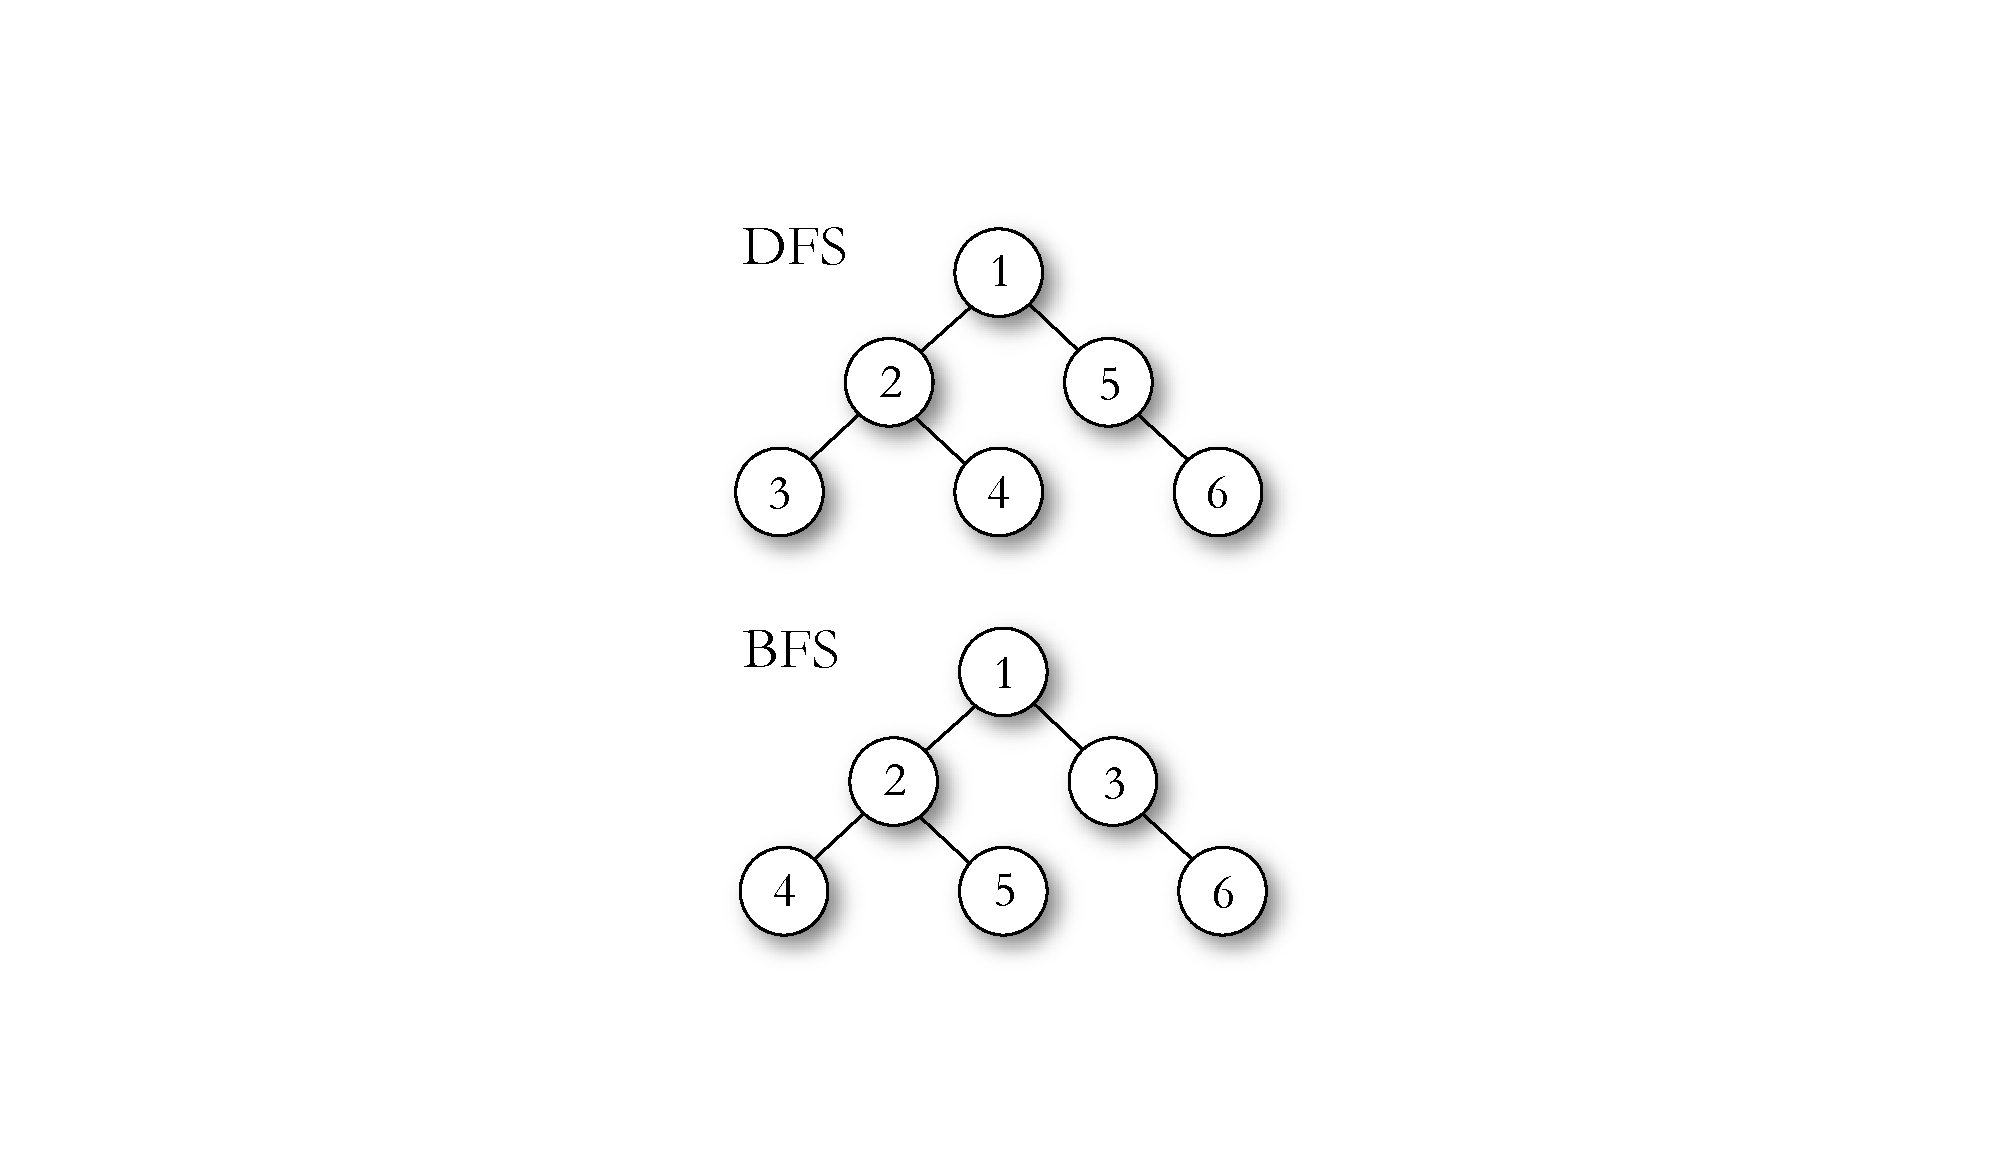
\includegraphics[width=0.3\textwidth]{BFS_DFS_long}
	\captionspacefig \caption{Comparison of the order in which vertices are explored, using the breadth-first-search (BFS) and depth-first-search (DFS) algorithms, where vertex 1 is the root vertex.} \label{fig:BFS_DFS}
	\end{figure}
\else
	\begin{figure*}[!htbp]
	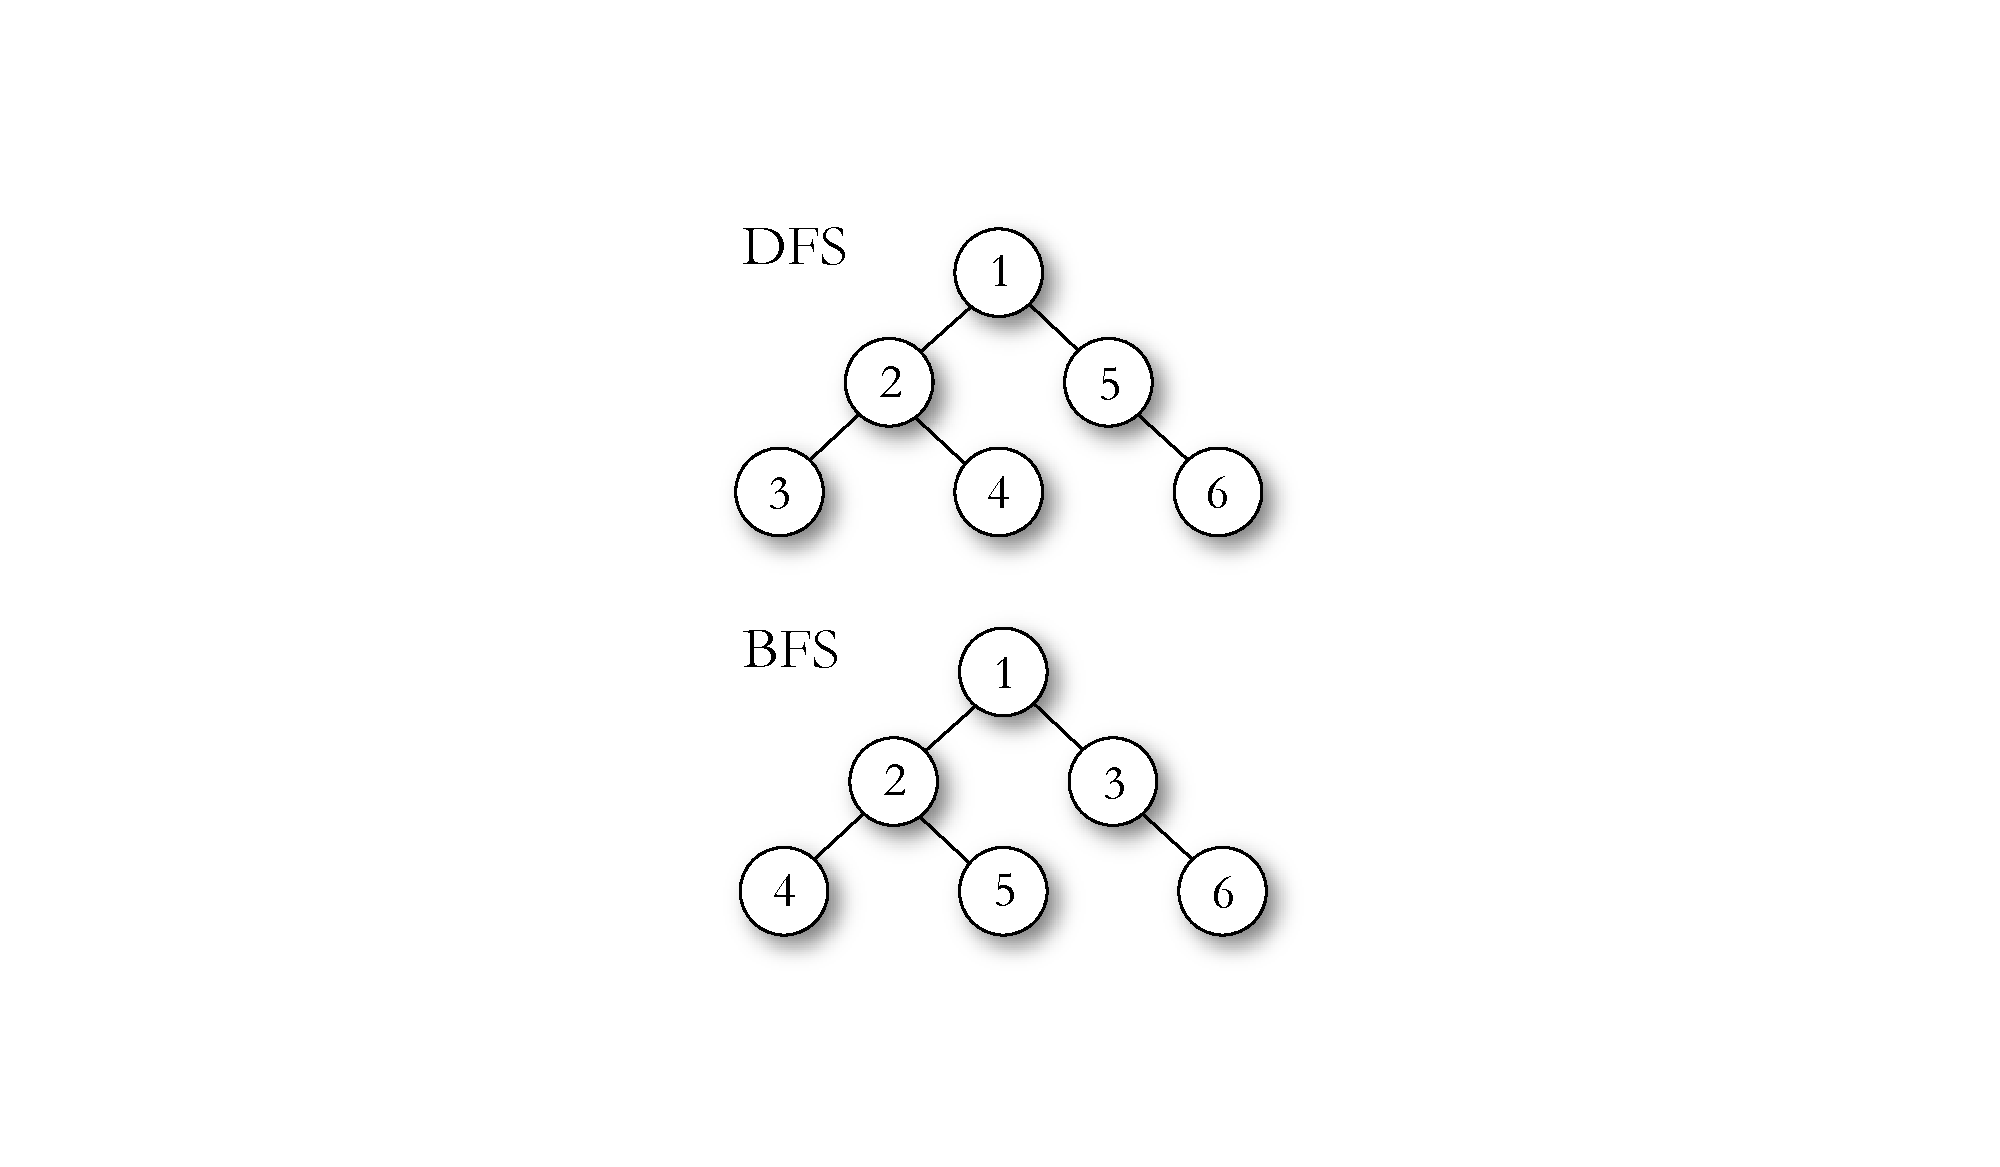
\includegraphics[width=0.65\textwidth]{BFS_DFS}
	\captionspacefig \caption{Comparison of the order in which vertices are explored, using the breadth-first-search (BFS) and depth-first-search (DFS) algorithms, where vertex 1 is the root vertex.} \label{fig:BFS_DFS}
	\end{figure*}
\fi

Both BFS and DFS guarantee visiting every vertex in a connected graph, and do so using only nearest neighbour transitions. Such algorithms are therefore very useful for network discovery.

The BFS algorithm is particularly applicable to pathfinding in ad hoc networks. Consider the situation where there is no central authority with full knowledge of the network, overseeing network operation. Rather, everyone needs to figure things out for themselves by only interrogating their neighbours, to whom they have direct connections. This directly leads to a BFS algorithm, where a node speaks to each of its neighbours in turn, who subsequently do the same thing, yielding a recursive algorithm. This can be naturally parallelised, as each node can be interrogating its neighbours independently, thereby implementing a distributed BFS algorithm. Note that, when searching for a target node, while the BFS algorithm obviously finds the target using the smallest number of hops (i.e a lowest-order route), it needn't necessarily find the route with the lowest cost (which is distinct from the number of hops in general). Shortest-path algorithms require a priori knowledge of the full network graph, discussed in Sec.~\ref{sec:shortest_path}.

Both BFS and DFS exhibit runtime	,
\begin{align}
	O(|V|+|E|),
\end{align}
where $|V|$ and $|E|$ are the number of vertices and edges respectively. Thus, these graph exploration algorithms reside in the complexity class \textbf{P}, and are classically efficient.

%
% Shortest-Path
%

\subsection{Shortest-path} \label{sec:shortest_path} \index{Shortest-path algorithm}

In graph theory, the shortest-path problem is that of finding a subgraph of a given graph $G$, connecting two vertices, \mbox{$A\to B \subset G$}, such that the sum of its edge weights is minimised. In the context of our application to route-finding, this amounts to finding a route that minimises cost.

The first proven shortest-path algorithm was invented by and named after Dijkstra \cite{bib:Dijkstra59}, which requires runtime,
\begin{align}
	O(|V|^2),
\end{align}
also residing in \textbf{P}\index{P} (one of the relatively few, and highly valuable optimisation problems that is classically efficient). Subsequently, a number of improvements and variations on Dijkstra's algorithm have been proposed, most notably the $A^*$ algorithm \cite{bib:Astar}\index{Shortest-path algorithm}, which has found widespread modern use, using a heuristic approach to improve performance over Dijkstra.

Formally, let $\vec{R}$ be the set of all routes \mbox{$A\to B$}. Then,
\begin{align}
c_\mathrm{opt} = \min_{r\in R} \left(\sum_{i\in r} c_\mathrm{net}(i) \right),
\end{align}
where \mbox{$i\in r$} denotes the $i$th edge in the route $r$. Intuitively, the (in general) exponential number of possible paths through a graph might lead one to believe the above optimisation problem is a computationally inefficient one (such as \textbf{NP}-complete, or worse). However, perhaps surprisingly, Dijkstra's algorithm cleverly manages to reduce this to a polynomial-time problem. A sketch of the algorithm is provided in Alg.~\ref{alg:dijkstra}, which needn't be understood by the reader desperate to read further.

\begin{table}[!htbp]
\begin{mdframed}[innertopmargin=3pt, innerbottommargin=3pt, nobreak]
\texttt{
function DijkstraShortestPath($G$,$A$,$B$):
\begin{enumerate}
	\item currentNode = $A$
    \item tentativeDistances[$A$] = 0
    \item tentativeDistances[others] = $\infty$
    \item nodesVisited[$A$] = True
    \item nodesVisited[others] = False
    \item loopStart:
    \item neighbours = currentNode.neighbourhood
    \item nodesVisited[neighbours] = True
    \item for(n$\in$neighbours) \{
    \setlength{\itemindent}{0.2in}
    \item newTentativeDist = \\ min(tentativeDistances[currentNode] \\+ edgeWeight[currentNode,n],\\
        tentativeDistances[n])\\
    \item nodesVisited[currentNode] = True
    \setlength{\itemindent}{0in}
    \item \}
    \item if(nodesVisited[$B$] = True) \{
    \setlength{\itemindent}{0.2in}
	\item return(tentativeDistances[$B$])
	\item $\Box$
    \setlength{\itemindent}{0in}
    \item \}
	\item currentNode = \\
	tentativeDistances[unvisitedNodes].\\
	nodeWithSmallest()
	\item goto(loop)
    \item $\Box$
\end{enumerate}}
\end{mdframed}
\captionspacealg \caption{Dijkstra's original shortest-path algorithm for finding the lowest weight path through a graph, $G$, between two vertices, $A$ (source) and $B$ (destination). The algorithm has $O(|V|^2)$ runtime (in \textbf{P}).} \label{alg:dijkstra}\index{Shortest-path algorithm}
\end{table}

Fig.~\ref{fig:simp_route_opt} illustrates a directed, edge-weighted graph. A shortest-path algorithm applied between vertices $A$ and $B$ would return \mbox{$R_\mathrm{shortest} = A\to F\to B$} as the minimum cost route.

When introducing network graphs earlier, we insisted upon all costs being associated with edges rather than vertices, and presented a trivial means by which to convert vertex costs to edge costs in Fig.~\ref{fig:remove_nodes}. This adamance arose because the presently described shortest-path algorithms operate purely in terms of edge weights, not vertex weights. But the mapping we presented from the latter to the former obviates this issue.

This is the motivating factor behind representing network graphs purely in terms of edge weights (Sec.~\ref{sec:quant_proc_in}), thereby enabling compatibility with shortest-path algorithms.

For the purposes of the QTCP protocol, we are interested in the case of directed graphs (recall that in terms of cost metrics, undirected graphs can be converted to directed graphs by replacing undirected edges with a pair of identical edges in opposite directions).

Shortest-path techniques find widespread application in many areas. Computer networks are an obvious candidate, since networks are inherently graph-theoretic by nature.

To implement the shortest-path algorithms discussed above, the party performing the calculation requires knowledge of the full network graph. In an ad hoc network, where users might be added to or removed from the network arbitrarily, this isn't necessarily the case.

One solution is for a central authority to be responsible for maintaining a ledger of all network participants and their connectivity, which users are required to notify upon joining or leaving the network. The central authority may then apply shortest-path calculations, which may be queried by users. However, a disruption in connection to the central authority, or failure of nodes to notify the central authority upon joining or leaving the network, introduces a point of failure into the operation of the protocol.

Another approach, which does not require a reliable central authority, is for users to implement network exploration algorithms each time they wish to perform a shortest-path calculation. This facilitates truly ad hoc networking, but incurs the cost overhead associated with nodes frequently implementing network exploration. However, network exploration is a purely classical algorithm, which may run entirely over the classical network, and therefore incurs no cost in quantum resources.

With this approach, a new node can join the network, without having to know anything about the topology of the network. Similarly, upon leaving the network, it needn't notify anyone, since a future interrogation by a neighbour will be detected as a non-existent node. The BFS is therefore highly suited to ad hoc operation. In fact, present-day internet gateway protocols (Sec.~\ref{sec:gateway}) essentially implement a distributed version of BFS.

%
% Constrained Shortest-Path
%

\subsection{Constrained shortest-path}\label{sec:const_short_path}\index{Constrained shortest-path algorithm}

In some scenarios we may wish to find a shortest-path through a graph, subject to some constraints. In general, the addition of constraints can make such algorithms far more computationally complex, undermining the efficiency of Dijkstra's algorithm. However, in some circumstances such constraints can easily be incorporated, without undermining the performance of the algorithm.

In particular, if there are constraints on the relationships between nearest-neighbours in the graph, this can be incorporated by pre-processing the graph via deletions of edges that violate the constraints. Then the usual shortest-path algorithm may be applied to the reduced graph. The rather trivial algorithm is shown in Alg.~\ref{alg:const_short}, with a simple example shown in Fig.~\ref{fig:constrained_shortest_path}.

\begin{table}[!htbp]
\begin{mdframed}[innertopmargin=3pt, innerbottommargin=3pt, nobreak]
\texttt{
function ConstrainedShortestPath($G$,$A$,$B$,$C$):
\begin{enumerate}
	\item For the set of nearest-neighbour constraints $C$, generate the set of edges $E(C)$ that violate the constraints.
	\item $G'=G-E(C)$
	\item route = DijkstraShortestPath($G'$,$A$,$B$)
	\item return(route)
    \item $\Box$
\end{enumerate}}
\end{mdframed}
\captionspacealg \caption{Efficient algorithm for finding a constrained shortest-path, where the constraints are in terms of nearest-neighbour relationships.} \label{alg:const_short}\index{Constrained shortest-path algorithm}
\end{table}

\if 2\pubmode
\begin{figure}[!htbp]
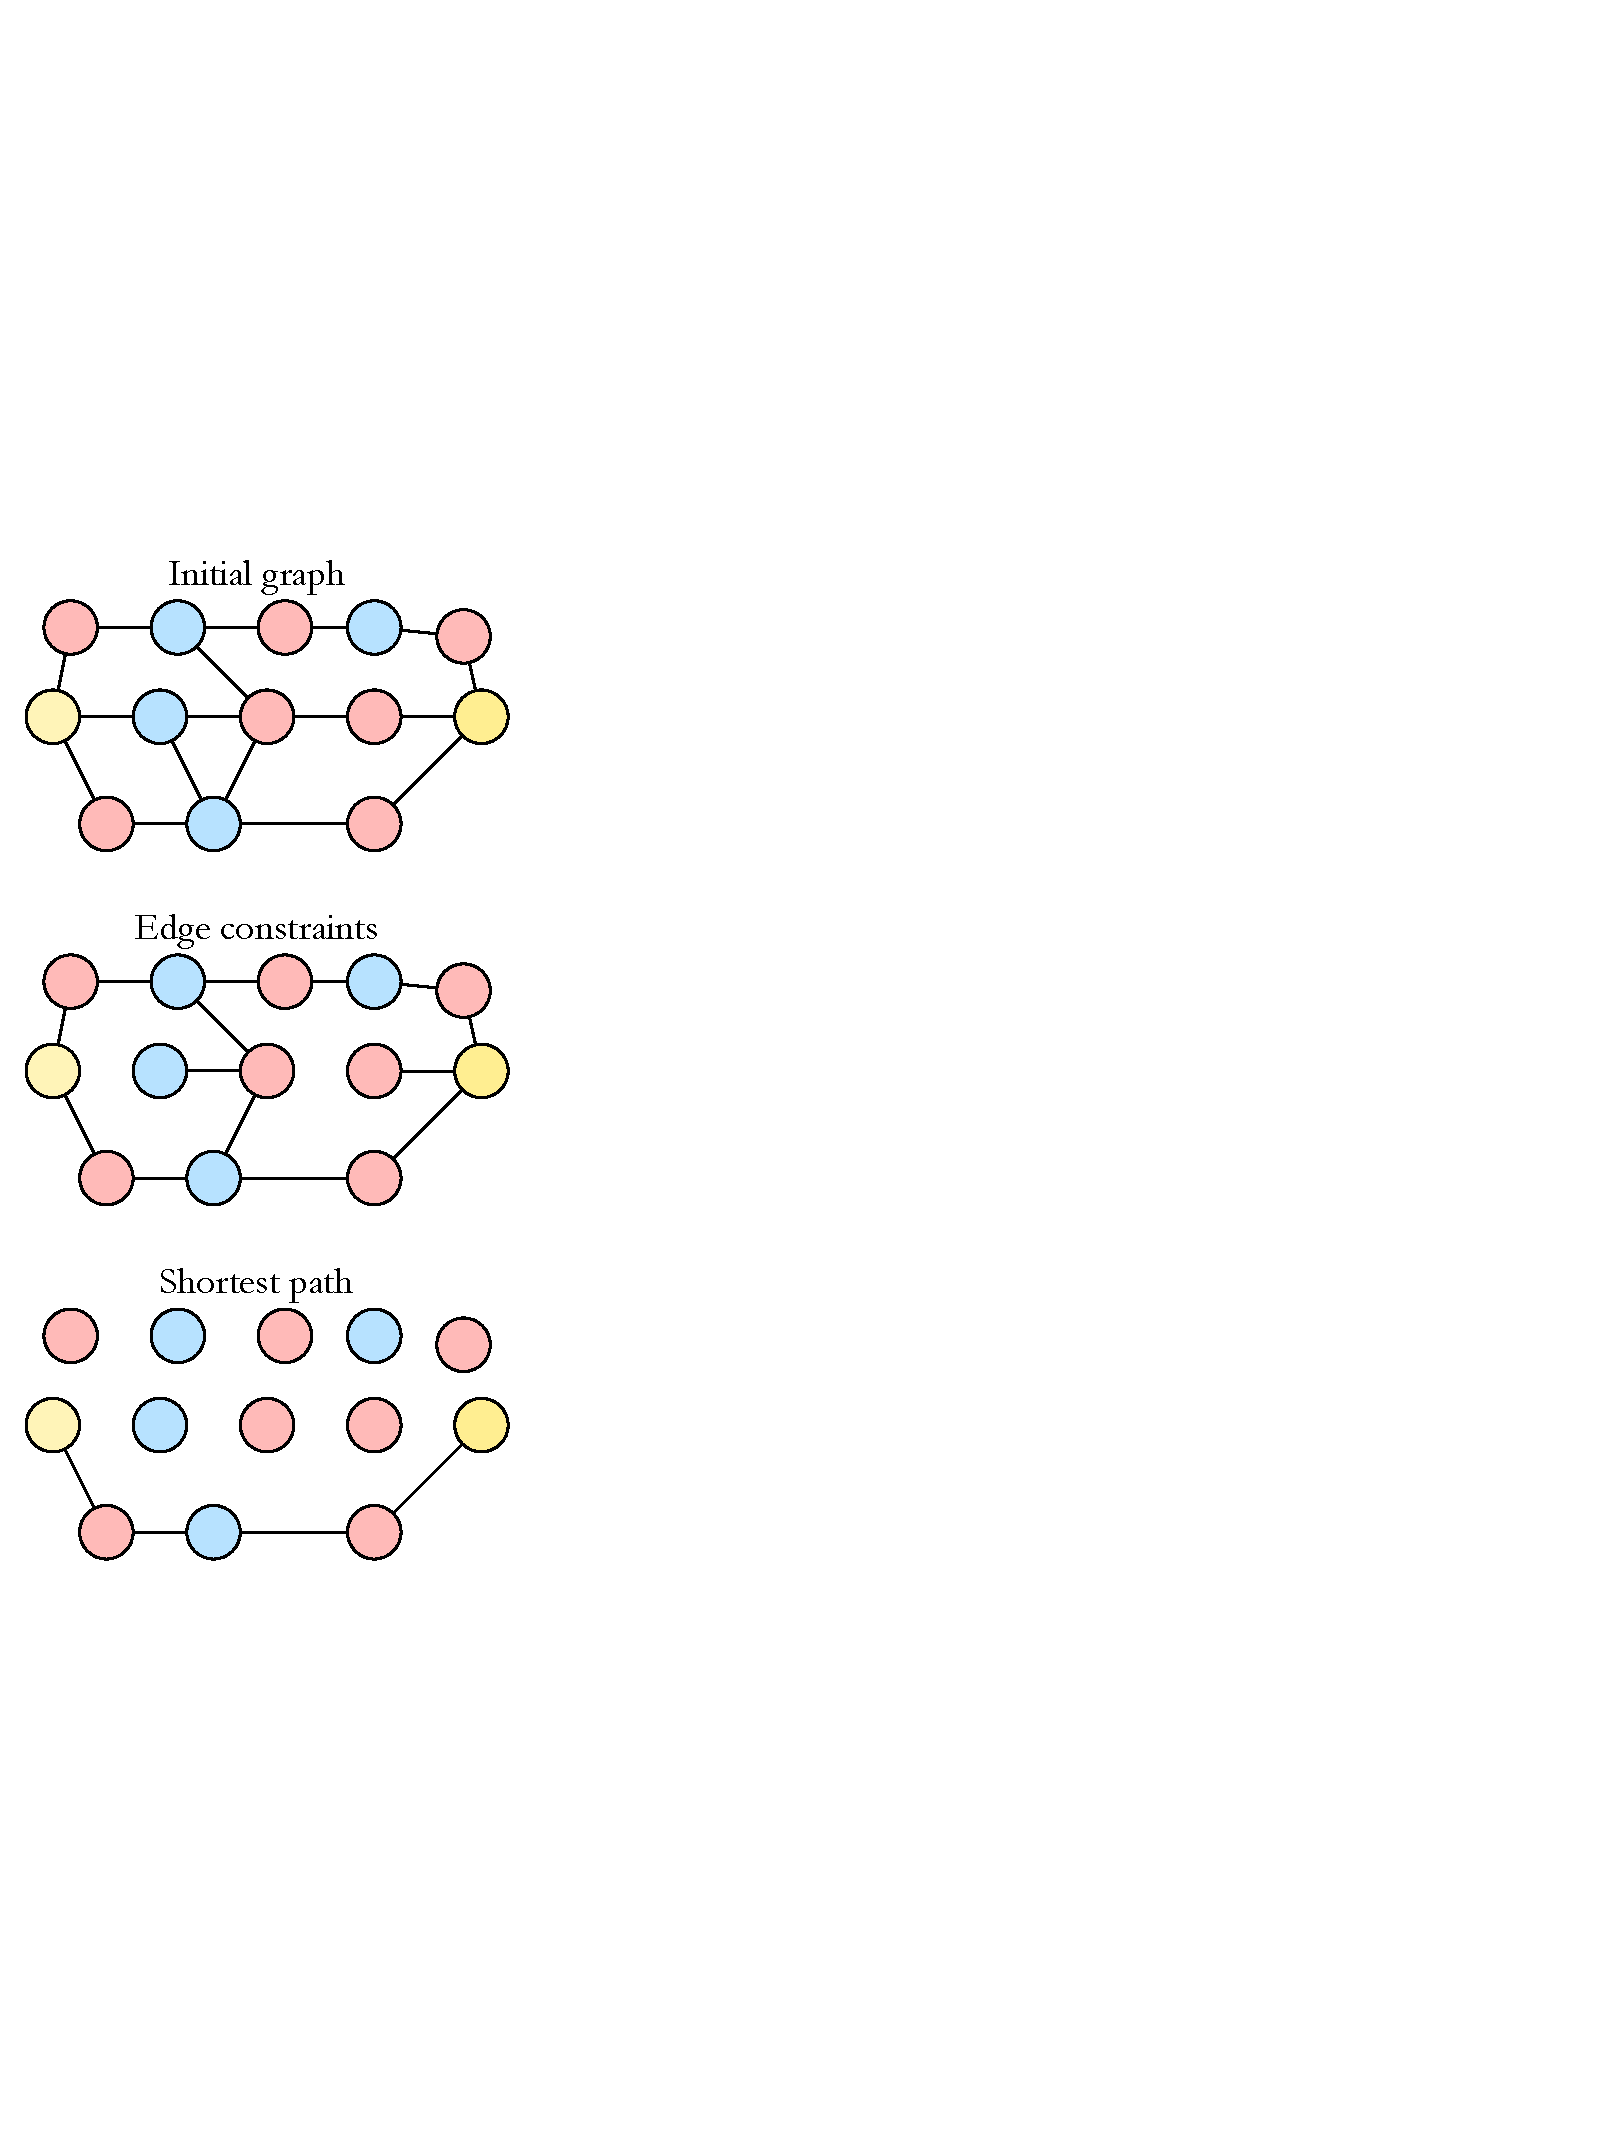
\includegraphics[width=0.35\textwidth]{constrained_shortest_path_long}
\caption{Example of a constrained shortest-path algorithm. Beginning with the initial graph we eliminate edges that do not satisfy imposed nearest-neighbour constraints. This is performed as a pre-processing stage. Then a usual shortest-path algorithm is applied to the reduced graph, yielding the optimal route subject to the required constraints.}\label{fig:constrained_shortest_path}
\end{figure}
\else
\begin{figure*}[!htbp]
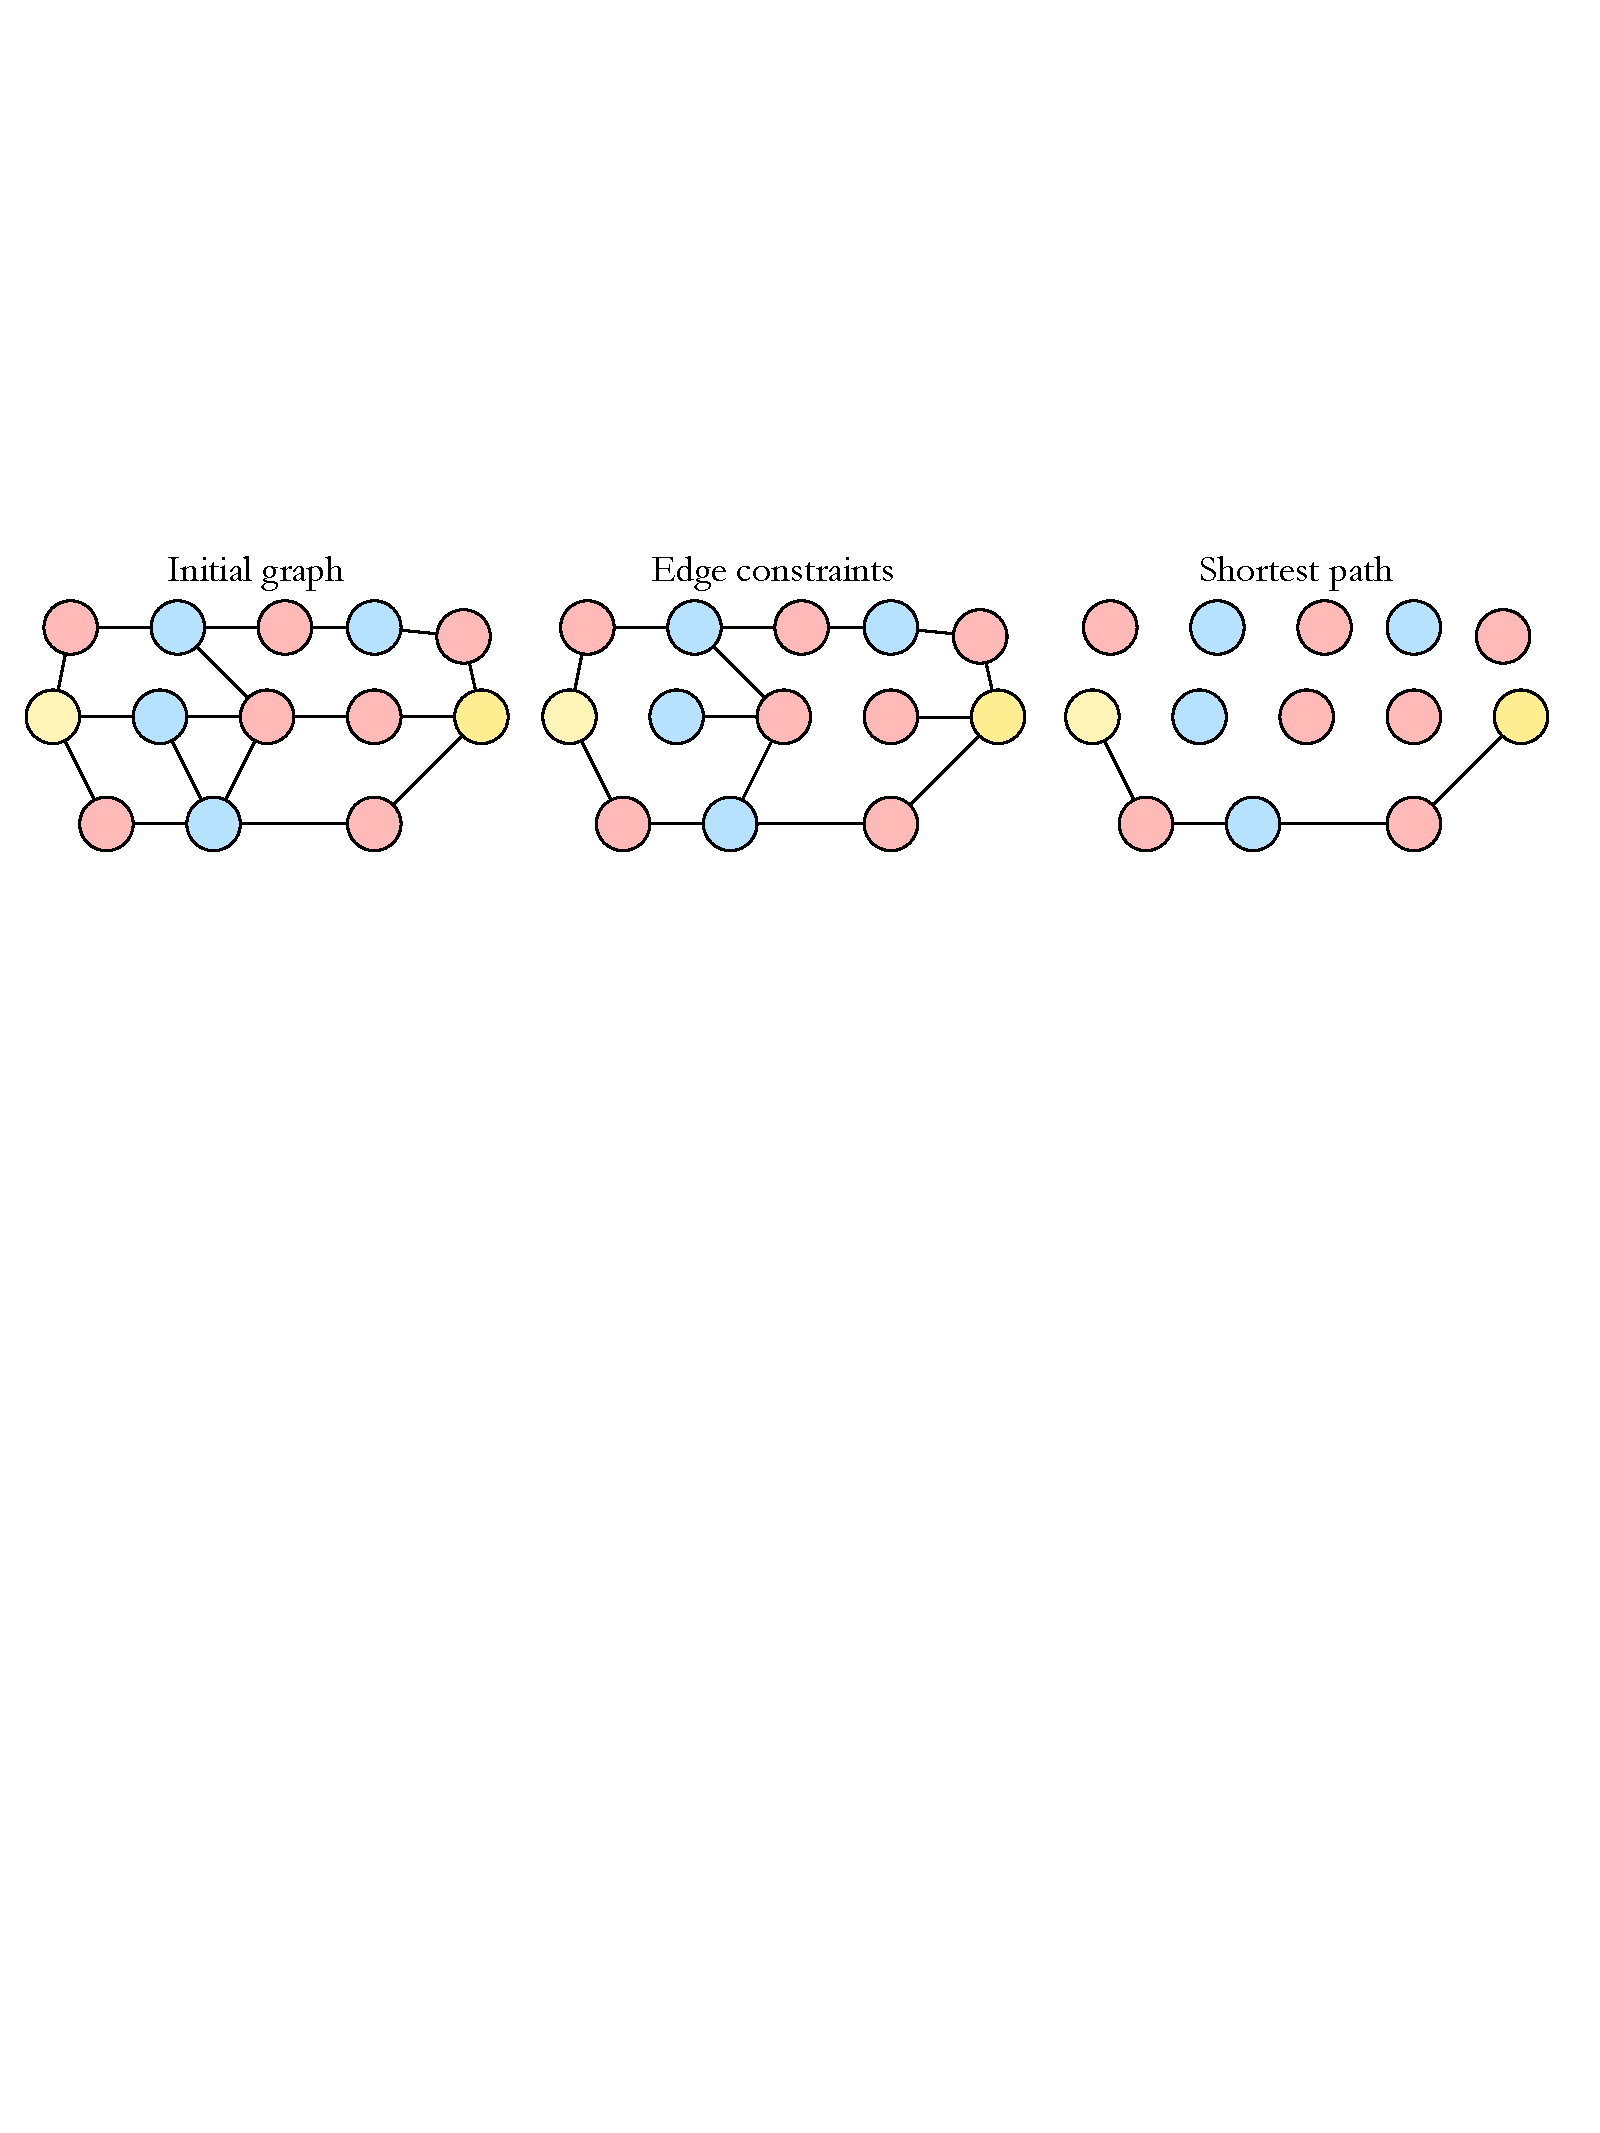
\includegraphics[width=\textwidth]{constrained_shortest_path}
\caption{Example of a constrained shortest-path algorithm. Beginning with the initial graph we eliminate edges that do not satisfy imposed nearest-neighbour constraints. This is performed as a pre-processing stage. Then a usual shortest-path algorithm is applied to the reduced graph, yielding the optimal route subject to the required constraints.}\label{fig:constrained_shortest_path}
\end{figure*}
\fi

A notable example of where this technique finds applicability is in entanglement swapping networks, discussed later in Secs.~\ref{sec:swapping} \& \ref{sec:rep_net}. Consider the network shown in Fig.~\ref{fig:racetime}. Here the entanglement swapping network comprises nodes alternating between two different functionalities: Bell-pair preparation, and entanglement swapping. Representing these as colours, this effectively introduces the edge constraint that edges between nearest neighbours of the same colour ought to be removed. Additionally, the end-points of the network must neighbour Bell-pair sources, not entanglement swappers. This enforces the additional constraint of removing edges between end-points with the wrong coloured neighbours. Having applies these edge deletions enforcing these constraints, the shortest-path algorithm will now find the constrained optimal route. Thus, this example of an entanglement swapping network is isomorphic to the example presented in Fig.~\ref{fig:constrained_shortest_path}.

%
% Single-Source Shortest-Path Algorithm
%

\subsection{Single-source shortest-path} \label{sec:single_source_sp} \index{Single-source shortest path algorithm}

The shortest-path algorithm by Dijkstra presented above finds the shortest route between two specified nodes in a network. However, when employing \textsc{Individual} routing strategies, where there is no central mediation of the network, each node desires an up-to-date routing table, showing the best route to take to any other point in the network. Then, upon receiving packets with particular destinations, rather than repeatedly applying Dijkstra's algorithm, we can simply look up the destination on the node's local routing table.

Single-source shortest-path algorithms address this problem by calculating the shortest paths from the current node to \textit{every} other node in the network topology.

The best-known algorithm for this problem is the Bellman-Ford (or Bellman-Ford-Moore)\index{Bellman-Ford-Moore algorithm} algorithm \cite{BF}, which requires worst-case runtime of,
\begin{align}
	O(|V|\cdot |E|).
\end{align}
Clearly this is more complex than Dijkstra's algorithm for finding a particular shortest-path. But it is more efficient than using brute-force to find the shortest-path between every pair of nodes in the network via $O(|V|^2)$ repeated applications of Dijkstra.

%
% Minimum Spanning Tree
%

\subsection{Minimum spanning tree} \label{sec:min_tree} \index{Minimum spanning tree algorithm}

MST algorithms find an MST\footnote{There may be multiple distinct MSTs for a given graph.} of some arbitrary graph. Like the shortest-path problem, it has a polynomial-time, deterministic algorithm (i.e it resides in \textbf{P}\index{P}). The first MST algorithm \cite{bib:Boruvka26} required,
\begin{align}
	O(|E|\log |V|),
\end{align}
runtime. Numerous variations have since been proposed, with little change to the underlying scaling.

Because MST algorithms are efficient, they play a very useful role in the design of real-world network topologies, where resource minimisation is crucial.

Fig.~\ref{fig:mst} shows an example of a graph with its MST.

%
% Minimum Cost Flow
%

\subsection{Minimum cost flow} \label{sec:min_cost_flow_prob} \index{Minimum cost flow algorithm}

The \textit{minimum cost flow problem} \cite{???} is that of minimising costs through a network for a specified amount of flow (i.e total bandwidth or throughput), which acts as a constraint on the problem. The definition of `cost' in this context is compatible with our earlier definition of cost metrics (Def.~\ref{def:metric}).

This problem can be efficiently solved using linear programming. Specifically, cost metrics along links in series are given by linear combinations of individual link costs. If, in addition, we let our net cost function be linear in the constituent costs then the net cost will also be linear in all the edge weights. This lends itself directly to optimisation via linear programming techniques. Algorithms for linear programming, such as the \textit{simplex} algorithm, have polynomial-time solutions (i.e reside in \textbf{P}\index{P}), and a plethora of software libraries are available for implementing them numerically.

One polynomial-time algorithm, by \cite{JAMES_B_ORLIN}, for solving this problem does so in, 
\begin{align}
	O(|V|\log |V|(|E|+|V|\log |V|)),
\end{align}
time.

%
% Maximum Flow
%

\subsection{Maximum flow} \label{sec:max_flow_prob} \index{Maximum flow algorithm}

The \textit{maximum flow problem} \cite{???} is the seemingly simple goal of -- as the name suggests -- maximising network flow, without consideration for any of the other cost metrics or attributes associated with the network. This type of problem is relevant when brute bandwidth is the dominant goal.

This problem can be tackled using a number of techniques. In some circumstances, linear programming techniques can be employed. The best-known algorithm is the Ford-Fulkerson algorithm\index{Maximum flow algorithm} \cite{???}, which finds a solution in,
\begin{align}
	O(|E|\cdot c_\mathrm{max}),
\end{align}
runtime, where $|E|$ is the number of links in the network and $c_\mathrm{max}$ is the maximum cost present in the network. The algorithm behaves pathologically in some conditions, which can easily be overcome in the context we present here. Using Ford-Fulkerson as a starting point, numerous other more sophisticated algorithms have been developed.

%
% Multi-Commodity Flow
%

\subsection{Multi-commodity flow} \label{sec:multi_comm_flow} \index{Multi-commodity flow algorithm}

The \textit{multi-commodity flow problem} \cite{???} generalises the previous algorithms to be applicable to multi-user networks. The generalisation is that there may be a number of distinct senders, residing on different nodes, each transmitting to distinct recipients, residing on different nodes. This is the most realistic scenario we are likely to encounter in a real-world quantum internet, where networks will inevitably be shared by many users, residing at different nodes.

Unfortunately the computational complexity of solving this problem is much harder than the previous algorithms in general. Specifically, solving the problem exactly is \textbf{NP}-complete\index{NP \& NP-complete} in general. However, in specific circumstances it can be approached using linear programming or polynomial-time approximation schemes.

%
% Vehicle Routing Problem
%

\subsection{Vehicle routing problem} \label{sec:VRP} \index{Vehicle routing problem}

The vehicle routing problem (VRP) is a multi-user generalisation of the shortest-path problem, where the goal is to minimise total network cost (i.e the sum of all individual users' costs) when there are multiple users sharing the network, each with distinct sources and destinations.

Unlike the polynomial-time shortest-path algorithm, exactly solving the VRP is \textbf{NP}-hard\index{NP \& NP-complete} in general. However, heuristic methods can find approximate suboptimal solutions far more efficiently, and there is a multitude of software packages available for doing so.

The VRP has found widespread use in, for example, the routing of transport networks for delivery companies or public transportation networks (hence the name), and many commercial companies exist, which perform these kinds of optimisations on behalf of transport providers to enhance their efficiency.

It is obvious that this algorithm is directly applicable to multi-user communications networks, which are conceptually identical to transport networks, albeit a bit faster. 

A multitude of variations on the VRP exist, accommodating for different types of constraints (or additional flexibilities) in the operation of the network.

%
% Vehicle Rescheduling Problem
%

\subsection{Vehicle rescheduling problem} \label{sec:VRSP} \index{Vehicle rescheduling problem}

The vehicle rescheduling problem (VRSP) generalises the VRP to the case where properties of the network undergo changes dynamically within the course of transmissions over the network. To use the analogy of transport networks, this could entail, for example, a truck breaking down en route to its destination, requiring real-time rescheduling of the other vehicles.

Solving the VRSP exactly is \textbf{NP}-complete\index{NP \& NP-complete} in general, but as with the VRP, heuristic methods can often be applied, which efficiently find approximate solutions.

In the context of communications over networks, the VRSP has obvious applicability -- a quantum internet is likely going to be largely ad hoc in nature, with users coming and going, and many non-deterministic points of failure, requiring ongoing updating of routing decisions if resource allocation is to remain as efficient as possible.

%
% Improving Network Algorithms Using Quantum Computers
%

\subsection{Improving network algorithms using quantum computers} \index{Network algorithms on quantum computers}

Given that we are directing this work at the upcoming quantum era, where quantum computing will become a reality, it is pertinent to ask whether quantum computers might improve the aforementioned network algorithms, some of which are computationally hard problems. Most notably, several of the discussed algorithms are \textbf{NP}-complete\index{NP \& NP-complete} in general, a complexity class strongly believed to be exponentially complex on classical computers. Can quantum computers help us out here, and improve network resource allocation? Can quantum computers help themselves?

While it is not believed that quantum computers can efficiently solve such \textbf{NP}-complete\index{NP \& NP-complete} problems, it is known that they can offer a quadratic speedup using Grover's unstructured search algorithm. Specifically, \textbf{NP}-complete\index{NP \& NP-complete} problems can be treated as satisfiability problems, where we are searching for an input to a classical algorithm that yields a particular output.

To gain a quantum advantage, we treat the classical algorithm as an oracle whose input configurations form an unstructured search space. Then, Grover's algorithm can perform a search over the space of input configurations to find a satisfying solution, with quadratically enhanced runtime.

While a quadratic improvement is far short of the exponential improvement we might hope for, Grover's algorithm is known to be optimal for the unstructured search problem \cite{?}. Nonetheless, despite only yielding a quadratic improvement, a quadratic speedup may already be sufficient to significantly improve network resource allocation.